60. \begin{figure}[ht!]
\center{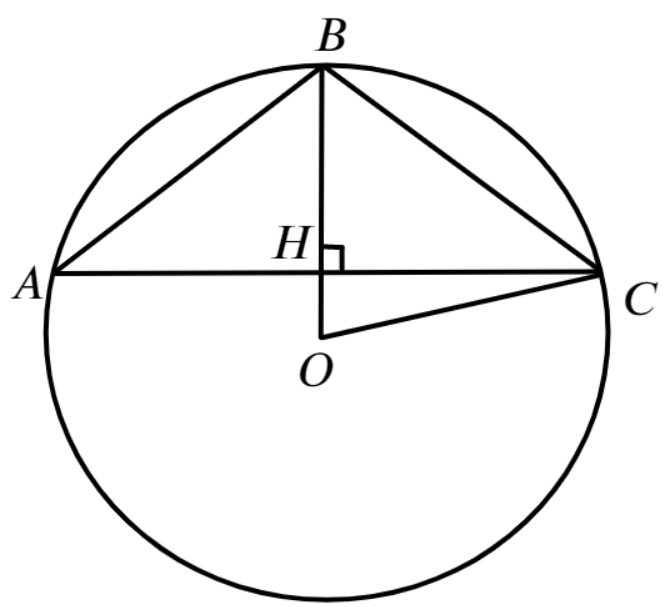
\includegraphics[scale=0.35]{g9-60.png}}
\end{figure}\\
Центр описанной окружности тупоугольного треугольника лежит снаружи. Найдём $BH=BO-OH=2-1=1$ и $HC=\sqrt{2^2-1^2}=\sqrt{3},\ AC=2HC=2\sqrt{3}.$ Тогда $S=\cfrac{1}{2}\cdot1\cdot2\sqrt{3}=\sqrt{3}.$ Выразим $AB=BC=\sqrt{1^2+(\sqrt{3})^2}=2.$ Площадь также можно найти по формуле $S=pr=\cfrac{2+2+2\sqrt{3}}{2}r=(2+\sqrt{3})r.$ Значит, $r=\cfrac{\sqrt{3}}{2+\sqrt{3}}=\cfrac{\sqrt{3}(2-\sqrt{3})}{4-3}=2\sqrt{3}-3.$\\
